\documentclass[11pt]{article}
\usepackage[top=1.00in, bottom=1.0in, left=1.1in, right=1.1in]{geometry}
\renewcommand{\baselinestretch}{1}
\usepackage{graphicx}
\usepackage{natbib}
\usepackage{amsmath}
\usepackage{hyperref}
\usepackage{todonotes}

\def\labelitemi{--}


\begin{document}
\bibliographystyle{/Users/Lizzie/Documents/EndnoteRelated/Bibtex/styles/besjournals}
\renewcommand{\refname}{\CHead{}}

\title{Effects of phenology on plant community assembly and structure }
\author{Elsa E. Cleland* \& E. M. Wolkovich*}
\date{\today}
\maketitle
\tableofcontents


\setlength{\parindent}{0cm}
\setlength{\parskip}{5pt}
*Authors contributed equally.

% Note to Lizzie: Check for TODO notes throughout. 
% One figure idea below (on traits), but really want on contrasting life histories



\section{Text in need of a home}

\emph{Definition to fit in ...} 
% timing of recurring growth and reproductive events (Ackerly)
% Isabelle is more of the `timing of recurring life history events ilk' and she stressed the seasonality of phenology as needing to be in the definition, but then we discussed tropical phenology etc. and she came around to this.
We define phenology as the timing of critical stages of growth and reproduction and the transitions between them. This definition is intentionally more inclusive than some other definitions, which focus on recurring or seasonal events, and thus can narrow phenology to only certain plant types or biomes (e.g., woody species in the temperate zone). This artificial narrowing to us can preclude understanding the selective pressures on phenology that---as we outline below---are critical for understanding the role of phenology in community assembly. Our definition thus includes both tree leafout, and seed germination of annual plants at the same time in encompasses fruiting, flowering and importation transitions in and out of these phases, such as dormancy and vernalization.

Phenological `events' are rarely one moment in time ... get into distributions and plasticity here? Or leave it where I have it below?

\emph{Text on frost and other traits ...} 
In many systems, spring frost is likely a controller on phenology that could lead to trait correlations. In most temperate and boreal systems freezing temperatures limit growth throughout part of the year, shaping the spring phenology of most species. Leafing or flowering before the last spring frost can mean losing tissue to frost, but simply pushing all phenological events well after frost though has its own costs as it means higher competition for light and other resources. This temporal landscape of shifting frost risk and competition predicts early species should have traits that allow them to cope with frost, but be competitively inferior under low resource conditions, while later species should show the reverse. Recent reviews suggest some evidence for this \citep{wolkovich2014aob,memegan2021}, but few have directly tested traits related to frost tolerance and avoidance, possibly because of the diversity of ways early-active species can deal with frost \citep{frostbook}. Species vary in what temperatures can cause tissue damage \citep{Lenz2013}, but universally tissues are most vulnerable during budburst and leafout \citep{frostbook,cat2019} thus species often have a suite of other mechanisms including waxy or hairy leaves to slow ice formation, rapid budburst to speed through the most dangerous period or cheap-to-build tissues so that tissue lost can be quickly replaced. This last mechanism fits neatly with a competition trade-off as leaf and vessel tissues that are easy to build are also those which generally cannot well compete for resources (ADDCITE). %TODO: Add Vitasse 'Earlier leaf-out rather than difference in freezing resistance puts juvenile trees at greater risk of damage than adult trees'

\section{Main text}

\emph{Introduction} 

Phenology, defined here as the timing of growth and reproductive events, is a key plant trait because it is often closely tied to the fitness of individuals in seasonal environments (\citet{verdu2005early}, \citet{munguia2011meta}). The timing of phenological transitions determines both the environmental conditions and biotic interactions experienced by individuals during different stages of their life-cycles (Donahue 2005), and hence the relative impact of these factors on survival and reproduction (Caruso et al. 2019). For instance, in temperate ecosystems, the timing of leaf emergence or flowering in spring can determine fitness consequences of frost events (Inouye 2008, Augspurger 2013), or the impacts of herbivores (Meineke et al 2021), on plant performance.

Plant phenology has also garnered global attention because observations suggest that phenology of many plant species has shifted in recent decades, associated with rising temperatures and co-occurring global changes (Wolkovich et al. 2012, Parmesan and Hanley 2015, Menzel et al. 2020). In response to experimental warming, plants generally display earlier spring events (e.g. leaf-out, flowering) and later fall events (e.g. senescence) (Stuble et al. 2021). However, there is considerable variation among species in their phenological sensitivity to both observed and experimental warming (Cook et al. 2012, Wolkovich et al. 2012). Species that track climate change by having greater plasticity for accelerated early-season phenology have been found to maintain or even increase their performance in experimental settings (Cleland et al. 2012), indicating that species-level phenological responses to global changes have the potential to influence process at the population- (Iler et al. 2021), community- (Cook et al. 2012, CaraDonna et al. 2014), and ecosystem (Piao et al. 2019) scales.

Phenology is one of many interacting traits that influence the suitability of an organism to its environment. Functional traits are at the core of many theories in community ecology (with the key exception of neutral theories, e.g. Hubbel 2005), especially those aiming to predict the assembly of local communities from a larger regional species pool. It is often assumed that plants have a suite of traits that determine their ability to survive and reproduce in different environments (Schimper 1903), and that traits also reflect strategies of resource-capture, such that species with similar traits will compete, leading to competitive exclusion during community assembly (Gauss 1932, MacArthur \& Levins 1967, Abrams 1983. Despite the recognized importance of phenology for understanding species responses to the environment, and structuring species interactions in communities, phenology is missing from many frameworks seeking to identify major axes of global plant trait variation (e.g. Westoby 1998, Wright et al. 2004, Diaz et al. 2015, Joswig et al. 2022). However, it has recently been recognized that phenology is essential in trait-based approaches to understanding species interactions, and community assembly (Cope et al. 2022).

Here we focus our review on the role that phenology plays in plant community assembly. We examine how phenology enters into major theories of community assembly, including the potential for phenology to influence competitive and facilitative interactions, and to shape priority effects. We also examine the role that phenology plays in life- history trade-offs, and how phenology shapes species co-existence. In addition to reviewing the theory, we review studies that document community assembly following disturbance, shifting community composition in response to global environmental changes, and the role that phenology plays in invasion by exotic species into resident communities, including efforts to assemble native communities that are resistant to invasion through restoration. We consider the role of multiple phenological transitions, including germination or seedling emergence, bud-burst or leaf-out, flowering, seed maturation and dispersal, and senescence.

Although evolutionary responses of phenology to changing conditions could play an important role in community assembly (e.g. Cavendar-Barres et al. 2019), we focus our review on ecological studies. To maintain our focus on community assembly, we have not included studies that focus on single species, nor on purely ecosystem-level measures of phenology. While trophic mismatch (Kharouba et al., 2018) is a potential outcome of shifting species phenology in response to global change, it is beyond the scope of this review. We also will not discuss how multiple global change factors interact to influence phenology (e.g. Zhou et al. 2023), nor the specific cues that underlie phenological transitions (e.g. Chuine \& Regniere, 2017). Although we may not yet understand the mechanisms by which different factors interact to influence plant phenology, the principles are well-discussed elsewhere.

\subsection*{Phenological assembly: From the abiotic to biotic environments}
% Section 2
% TODO: Need ref for Janneke 2012 review (HilleRisLambers et al.)
Communities assemble from a regional species pool through a series of abiotic and biotic sorting processes. At the largest scale, a community's assemblage is limited by species in the larger regional pool---species well suited to an environment may thus not appear in it unless they are present in the this regional pool. From this pool, species are filtered based on the abiotic environmental conditions of a particular location---species must be able to persist through an environments extremes in hot, cold, dry, wet and other factors to pass through this `environmental filtering' step of assembly. This collection of potential species that could form a community is then filtered once more---by the pool of species itself. 

Competitive, facilitative, predatory and all other biotic interactions determine which species together can co-occur in the long term. If two species compete too strongly, then only the stronger competitor will remain in the community at this step, and similarly obligate mutualists, predators and parasites will persist only if the other species they require are present in the community. This final stage of assembly is where much of community ecology has focused over its history as a subdiscipline, driving theories of coexistence, including whether species even truly `coexist' or merely are on a slow walk to extinction for all but one species in each community \citep{Hubbell:2001vo}. 

Phenology enters community assembly at both the environmental and biotic filtering steps. Species phenologies must match the environment to pass the first filter: their growth and reproduction must be timed to match periods when the environment is mild and resource-rich enough for these events. Thus, in an environment with cold sub-freezing winters, species generally must have well-timed dormancy to avoid leafing out in the middle of the winter when they would loose all new tissue. Similarly, arid and tropical environments impose filters against certain phenologies. Once a set of species pass the environmental filter, phenology matters again at the biotic filtering step, where species with too similar phenologies may compete too strongly to co-occur.  Alternatively, species that overalp phenologically have the opportuity to develop facilitative  interactions \citep{duchenne2021phenological} promoting co-occurrance, while species with little phenological overlap are unlikely to interact via biotic filtering processes.

These two steps at which phenology is relevant to community assembly suggest a simple temporal matching that obscures the underlying complexity of most phenological `events,' such as leafout or fruiting. First, while `event' suggest an almost instantaneous timepoint, this is gross simplification. Phenology is an attempt to extract and simplify the temporal dimensions of various developmental processes that can rarely if ever be one point in time. Instead, phenology is generally a series of distributions. For any one event within one individual, there is a distribution of the process starting, peaking and ending, which can be variously imagined as a normal curve or sigmoid curve (imagine the event of a grape cluster ripening: the number of berries ripening each day mapped over time, would look normal, while the progress towards all berries ripened would be sigmoid). This then scales up across individuals within a population, and across populations \citep{inouye2019}. Such complexity is generally simplified into an `event' that often represents the 50\% point extracted statistically after repeated observations. 

Second, phenology---as a point in time---can appear highly flexible or strongly fixed---depending on how time is defined. To date, much work has used calendar time for phenology: a snowdrop flowers on a certain day of the month in one year, for example. When measured this way, phenology appears highly flexible---jumping around in temporal space from year to year or place to place---as the environment is variously warm, cool, dry or wet. Yet, plant phenology can also appear highly deterministic when defined in biological time; that is, when defined as relative to a set of known environmental triggers, such as accumulated cool temperatures known to vernalize some flowering species. When the underlying triggers or cues for phenological events are fairly well understood for some events (with perhaps flowering in \emph{Arabidopsis thaliana} being the best understood) phenology can be highly predictable and effectively---inflexible. For the purposes of our review here, we cotton more to the latter interpretation which strips away complexities of geography that do not necessarily aid our understanding of phenology \citep{davies2013}. 

\emph{Where phenology fits in the environmental vs. biotic filtering part of community assembly}
% TODO: Check out Kraft thought piece (separating out biotic and env is almost impossible, focus on tolerance; in FuncEco), but also ask JD 

The importance of phenology to species passing the environmental filter of community assembly has been long studied---though rarely framed in exactly these terms. Early studies of the controls on species ranges stressed phenology as a major axis (CITES). Today process-based models based almost entirely on species phenology are highly predictive of tree species ranges \citep[where they have been tested,][]{chuineJTB,Morin:2009gt,morin2007}. These models integrate over both growth and reproduction: trees leafout, flower and fruit then lose tissue to frost if temperatures dip below their cold limits (which vary for leaves, flowers and fruit), they then must have a long enough season for fruit development. Various species in various range edge are limited by tissue damage, fruit ripening or carbon starvation---depending on the summed outcome of a phenological model. 

Range models based on phenology highlights the life history challenges of phenology---species must fit in a sequence of events to grow and reproduce within environmentally feasible periods. Through this lens, the sequence and length of phenological events becomes critical, and prevalent trade-offs from life-history theory become more relevant. For example, trade-offs between fruit size and growing season length may either drive or depend on whether species flower before they leaf, a still open question in plant biology \citep{dan2021nph}. [Similarly, something about iteroparity and semelparity ...?] These complexities are present in many process-based models, but rarely extend beyond into either life history or community ecology theories. Process-based models similarly view phenology often as a static trait that shapes broad-scale (biogeographical) processes, with little focus on the role it may play within communities. Yet plant invasions suggest this view is overly narrow.

Recent work on plant invasions suggest a role for phenology beyond simple environmental filtering. Theory in invasion biology focuses both on the characteristics of the species invading, and on the community into which it invades, with the vacant niche model proposing that species should invade if there is open `space' in a community and the invader fits that space. Phenologically, this predicts species not to simply filter in based on their phenological match to the abiotic environment, but on their match to the biotic environment. Invaders should thus take advantage of open temporal space within communities, which some evidence suggests they do---particularly at the start of seasons (see next section). 

Findings from invasion biology support a potential role of temporal niches more broadly in community assembly \citep{gotelli1996}. Static environments (e.g., a chemostat) cannot easily support temporal niches, but even slightly more complex dynamics of resource availability across a season can create the potential for temporal niches (Fig. \ref{fig:resource}). Models including a simple resource pulse that starts a growing season can theoretically create space for temporal niches and thus phenological assembly (discussed further in the section on coexistence). Such models, however, highly simplify the resource dynamics of most environments, which is more aptly described a multi-dimensional mosaic of access to light, water, and nutrients variously present through abiotic factors (weather, tree fall due to storms etc.) and lost through uptake and use by other species. This complexity leaves much room for the order of species arrival to matter .... 

\subsection*{Priority effects}

In addition to the roles of environmental filtering and biotic interactions for determining the temporal niches of species in assembled community, the relative timing of arrival of a species can influence community assembly through priority effects (\citet{alford1985priority}, \citet{chase2003community}, \citet{fukami2015historical}). Priority effects have often been considered as historical contingencies in the process of community assembly, arising from the chance establishment of individuals of different species, resulting in different community compositions across sites that are otherwise similar in terms of species pools, environmental conditions and disturbance histories (e.g. \citet{diamond1975assembly}). In the context of succession, early studies noted that the timing of disturbance relative to seasonality of seed dispersal could result in different species initially colonizing sites, and variation in later species abundances (\citet{keever1950causes}, \citet{holt1972effect}). More recently, it has been recognized that the relative order of species’ growth onset throughout the growing season can also greatly influence the relative abundance of species later in the season via priority effects (\citet{fukami2015historical}, \citet{wainwright2012seasonal}, \citet{rudolf2019role}).  Phenology is a key aspect of a species niche, and hence should be key to niche-based predictions of community assembly (\citet{vannette2014historical}).

The predictive power of priority effects for understanding community assembly suggests that the potential for competitive exclusion is not even across the growing season, and should drive patterns where phenologically earlier species are competitively dominant. For instance, the timing of germination is a trait which is highly linked to plant fitness, because it determines both the biotic and abiotic environment experienced by the emerging seedling (\citet{donohue2010germination}). Foundational studies demonstrated that earlier germinating individuals achieved higher adult size, likely via space and resource pre-emption, and competitive suppression of later germinating individuals of the same species (\citet{ross1972occupation}),  a type of asymmetric competition (\citet{connolly1996asymmetric}). . Subsequent work has found repeatedly that earlier germinating species gain a competitive advantage over later germinating species (\cite{cleland2015priority}, \citet{waterton2016trade}, \citet{blackford2020species}). Hence it is unsurprising that seeds can “sense” the presence of neighboring seeds, and display accelerated germination in more competitive environment (\citet{dyer2000accelerated}).

However, a number of factors can reduce the benefit of early germination phenology. For instance, apparency to herbivores (\citet{waterton2016trade}) or exposure to sub-optimal conditions such as early-season drought (\citet{wainwright2012seasonal})  can create trade-offs whereby later germinating species can achieve numerical dominance. Further, priority effects are not always competitive; experimental work with \textit{Arabadopsis thaliana }has shown that individuals germinating during stressful periods of the growing season can be facilitated by neighbors (\citet{leverett2017germination}). This finding is broadly consistent with the prediction that competitive priority effects will be stronger under conditions of high resource availability or low stress (\citet{vannette2014historical}), opening the door for facilitative priority effects to arise under stressful conditions.

Priority effects arising via differential germination timing are likely to be most important in herbaceous-dominated ecosystems, but may also arise in woody-dominated ecosystems via the timing of spring green-up, due to light pre-emption by species with earlier growth dynamics. For instance, the non-native Amur honeysuckle invades the understorey of deciduous forests in the Eastern U.S., where it has earlier leaf-out in the spring likely associated with greater frost tolerance compared with co-occurring native shrubs (McEwan et al. 2009). The potential for priority effects to arise directly from earlier season flowering are less clear mechanistically, and early-flowering species are more prone to frost damage in temperature ecosystems (\citet{inouye2008effects}). However, the timing of flowering can indicate of the timing of soil resource uptake, with important implications for community assembly \citet{gulmon1983phenology},\citet{seabloom2003invasion}.

Restoring native plant communities, and preventing invasion by exotic species, are two areas where phenological priority effects can play a key role in optimizing desired endpoints of community composition. Non-native species have sometimes been observed to germinate (\citet{wainwright2012seasonal}, \citet{wilsey2011biodiversity}) or flower (\citet{cleland2013strengthening}) earlier than co-occurring native species, suggesting phenological priority effects may be one factor predicting the successful establishment of invaders into resident communities (\citet{wolkovich2011phenology}, \citet{alexander2019earlier}). Priority effects can also be mediated by plant-soil feedbacks whereby earlier active invaders can change the environmental conditions for later active native species (\citet{grman2010within}). However, other reviews have found that phenological differences between invading and resident species are mediated by invader origin (\citet{godoy2009flowering}) or found limited evidence of phenological differences between native and non-native species (\citet{zettlemoyer2022limited}), and there have also been cases where later-active invaders that achieve greater size outcompete early-active native species (\citet{godoy2014}). Together these findings suggest that the role of phenology in community assembly inherently depends on how phenology correlates with other traits important for invasion.

In the context of restoration, introducing target native plants to a recently disturbed site either earlier in the season, or as larger plants rather than seeds, can give them a priority advantage over invasive species in the seedbank (Young et al. 2017, Wilsey et al. 2021). Experimental studies sometimes find that phenological priority effects of invasive species are stronger under conditions of nutrient encihment (\citet{kardol2013resource}, \citet{valliere2022phenological})  consistent with theoretical predictions (Vanette \& Fukami 2014), suggesting that restoration strategies to reduce soil nutrient availability (such as carbon additions) help reduce the seasonal priority effects of invading species on native communities (Cleland et al. 2012).

Climatic context is also likely to pay a role in phenological priority effects. Interannual climate variation (Levine et al. 2011) or directional changes in climate (Parmesan 2006) can change the relative order of species seasonal phenology, with resulting changes in species interactions and species relative abundances (Thomson et al. 2017, Buonaiuto \& Wolkovich 2023). Thus, seasonal priority effects likely play a key role in understanding changing species compositions in plant communities over time.

...
Priority effects can plan a major role in determining the likelihood of species co-existence, and have been incorporated into models of modern coexistence theory (Grainger et al. 2019, Godoy \& Levine 2014).

\subsection*{Phenological coexistence}

By defining the temporal niche, phenology links clearly to theories of species coexistence focused on niche partitioning. Decades of theory have posited that plant communities are organized by a final critical filter where each species uses a unique set of temporal, spatial and otherwise environmental resources (CITEhutchinson). This allows each species to be uniquely superior in one particular $n$-dimensional niche space and thus increases intra-specific competition above inter-specific competition---a critical component for species to coexist. Through differing vegetative phenologies, species could use the same exact resources but occupy distinct temporal niches and thus coexist. 

Coexistence through niche differences is often referred to as a `stabilizing mechanism' in the canon of what is now often called `modern coexistence theory' (citeCHESSON). Modern coexistence theory divides mechanisms of this final stage of community assembly into stabilizing mechanisms---which increase intra-specific competition relative to inter-specific and thus can contribute to coexistence through species differences---and equalizing mechanisms---which decrease fitness differences. Equalizing mechanisms generally reduce true coexistence, but can lead to apparent coexistence as two identical species will generally co-occur in nature for a very long time (until one is lost to stochasticity, citeHUBBEL). This canon has dominated coexistence research of recent decades and underpins recent work to integrate phenology.

A number of recent studies leverage niche differences to argue that phenology is critical to coexistence in plant communities. \citet{godoy2014} found that differences in phenology tended to increase niche differences in experimentally assembled grassland communities of native and exotic species, but this did not promote coexistence. Instead, the phenological uniqueness of some invaders promoted their invasion, while other invaders benefitted from an apparent correlation between phenology and competitive ability (later active species---both native and exotic---appeared competitive superior to early-active species). Correlated phenology and competition was also used by Rudolf 2019 (CITE) to insert phenology into classical coexistence equations for competing species. In this approach, increased phenological differences between competitors promote coexistence when the earlier species is the inferior competitor. \citet{memegan2021} apply a similar trade-off to show that a species attribute strongly related to phenology---`environmental tracking'---can be critical to coexistence when it trades off with how well species convert resources to new biomass. Most recently Levine 2022 (CITE) added phenology to classical coexistence equations by allowing species to have longer or shorter season; here coexistence is possible if phenology trades-off with a growth rate advantage---effectively a type of competitive advantage.  

As these studies highlight, recent research heralding the importance of phenology to coexistence all leverage a similar trade-off between phenology and competitive ability. Given the domination of competition in current coexistence theory and research, this seems the most obvious and natural point to insert phenology into coexistence. Superficially the idea that phenology and competition trade-off is very attractive: if species vary their overlap in time, they should compete less and reduced interspecific competition should increase stabilizing niche differences and promote coexistence, but this is not the exact angle these models are leveraging. Instead they posit that earlier or later species (depending on the model) are competitively superior (through one parameter or another) thus invoking a rather simple trade-off. This trade-off would work equally well for many plant traits; fundamentally any plant trait added to a classic competition model such that it trades off with competitive ability will promote coexistence through stabilizing niche differences. Our current insights into how phenology specifically effects coexistence is thus, still rather narrow and not terribly specific to phenology. 

These models also generally insert phenology as a coexistence mechanism mostly independent of environmental variation---even though phenology itself varies year to year with environmental variation. These current studies, like much of the work on modern coexistence theory focus on resource partitioning---a fluctuation-independent mechanism of coexistence---ignoring an additionally suite of likely relevant mechanisms that are fluctuation dependent: relative non-linearity of competition and the storage effect. While not yet tackled (to our knowledge) and certainly more complex to model and study, these two mechanisms seem highly relevant to phenology. Relative non-nonlinearity promotes coexistence through variation in competitive intensity over time or space, given that species have different nonlinear responses to competition \citep{CHESSON:1994vn,Chesson:2000vd}. Recent work suggests relative non-linearity may be an important and under-appreciated mechanism in plant communities, but attempted to `control' for phenology rather than consider it (Hallett). Yet species varying phenologies could produce varying competitive intensity over time and/or create the non-linear response. 

% [And they're missing the fun meat ... ] While most recent work on modern coexistence theory focuses on separating stabilizing and equalizing mechanisms, the theory also encompasses and overview of the three ways coexistence can occur: relative non-linearity, XX and the storage effect. 
% From Chesson 2000 'In the case of temporal fluctuations, these mechanisms can be divided into two broad classes: relative nonlinearity of competition and the storage effect.' and the other is mean fitness differences (according to my notes from working with Megan way back when).  You can check out: https://eeb.arizona.edu/chesson-lab which has links for fluctuation dependent (links to resource partitioning) and fluctuation independent mechanisms, which is handy. 
% Hallet cite: Rainfall variability maintains grass-forb species coexistence
Similarly, the underlying mechanisms of storage effect---where species vary in their responses to the environment, and that response covaries with competition---could clearly relate to phenology, as is often theoretically proposed \citep{Chesson:1993gi,Chesson:2004eo}, but rarely tested. Instead the storage effect today is generally tested on interannual timescales for annual plants, where the model prediction that species `store' environmentally favorable periods (`buffered population growth') can be tested through seedset. Older work focused on storage outside of seedbanks has made phenological predictions. \citet{Kubo:1996qe} generated a model of coexistence for tropical forest trees where species compete for spatial gaps---and their associated resources---at the start of climatically favorable periods each year. The model predicted phenological diversity across tree species that depended both on the length of climatically unfavorable periods and the phenological widths of species---effectively the size of the temporal niches \citep{Kubo:1996qe}. Storage occurred through long-lived adult stages, with seedbanks assumed to have weak dormancy (and thus could not provide `storage' of good environments). This approach contrasts in the method of storage compared to models today focused on annual plant communities, yet both approaches have similarly allowed storage through only one mechanism and focused on inter-annual timescales.

Yet the complexity of species phenologies and overall life histories makes it seems likely they may use more diverse timescales and multiple types of `storage'. (Just the way chinstrap penguins get in a good nights sleep through thousands of daily micronaps....)  Indeed the definition of `storage' in the storage effect model highlights this complexity---and unites varying life histories under one model---storage can be through seed banks, long-lived life stages in perennials, or through dormancy periods \citep{Chesson:2000vd}. Most plant communities contain a mix of these storage strategies across species, and within species multiple ways to store environmentally favorable periods seem common. Including this complexity in coexistence theory, however, likely requires modeling phenology as a more nuanced and complex trait. 

Models of the role of phenology in coexistence generally simplify phenology to a single trait that is rarely clearly linked to one or more events \citep[even when studied with empirical data][]{godoy2014} . Because phenology generally trades-off with resource competition in most models, events related to growth such as germination, or leafout seem likely candidates for some models \citep[e.g.,][]{godoy2014,memegan2021}, but others seem to implicitly model phenology as total growing period (CITEnewLevine). Most accurate to these models would be when resource uptake is greatest, which recent research suggests relates to phenology (CITEheberling), but perhaps not in ways that allow us to generalize from phenology to resource uptake across species (CITES). Further, most models appear to ignore reproductive events, such as flowering and fruiting, which occur before leafout for many species (CITE) and may play a large role in determining the timing of growth events (CITES). 

Within coexistence and more generally in phenological research, much work focuses on one event---erasing the complexity of phenological events that are all generally dependent upon one another. This is perhaps not surprising, as making predictions for sequences of events requires bridging from coexistence to life history theory, which has worked to predict the optimal schedule of growth and reproductive timing across an organism's lifetime. But recent work showing that differences in life history can lead to long-term persistence of species in an otherwise neutral model (where species are effectively equalized, CITE) suggests the lines between coexistence theory and life history theory perhaps could be quite usefully blurred. 

% And maybe something here on that they're missing predators and disease? ... 

\subsection*{Future directions}

% START here and try to write something exciting about life history versus community ecology ... ? (Incl. bet-hedging, geometric constraints etc.) Definitely ADD Cohen and Iwasa models of storage and how Yoh Iwasa used to work on both the optimal growth/reproduction and community assembly. 

{\bf All just notes for now...}
 how relevant this phenology x competitive ability  trade-off is in natural systems is debatable. 
 
 Advancing our understanding of how phenology fits within coexistence will likely involve a more head-on reckoning with the challenge of time in community assembly models ... STIFF equations here? 

% -ignoring an additionally suite of likely relevant mechanisms that are fluctuation dependent: relative non-linearity of competition and the storage effect. ... seem highly relevant to phenology and could yield new insights. 

Relevant fields overly focused on different plant life histories: coexistence focused on annuals and storage through seedbanks, while much phenology work focuses on trees and their recurring annual events. 

They do! Perhaps because phenology is such a critical component of life history, that once you add it to coexistence theory you are then embedded in life history theory -- but these fields are not meeting enough (but see new O'Dwyer paper in \emph{Nature}, which includes ``the schedule of birth, growth and death matters for predicting persistence time, even when fitness and niche differences are taken into account"). So Cohen 1976 (and Iwasa \& Cohen 1989) and other papers about optimality of transitions should be incorporated more into coexistence. 

Also, what do we need in coexistence theory? Models that include intra-annual and inter-annual dynamics and (1) figure out how three mechanisms of coexistence divide out between within and between seasons and how they might shift with warming. (2) Maybe partition what percentage of species co-exist due to what mechanisms should be a goal .... 

Make the point about intra-annual lottery model in paper: Coexistence theory had a phenological period, but it has basically been ignored by new work (see phenological segregation model of Kubo \& Iwasa 1996), which includes ``The result is closely related to the discreteness of the evolutionarily stable strategy in a pure-strategies lottery model studied by Sasaki and Ellner (1995)." 

\newpage
\section{References}
\bibliography{areesbib.bib}

\newpage
\section{Figures}

% Figure idea: Show shifting frost risk versus competitive environment and how that might correlate with traits? 

\begin{figure}[h!]
\centering
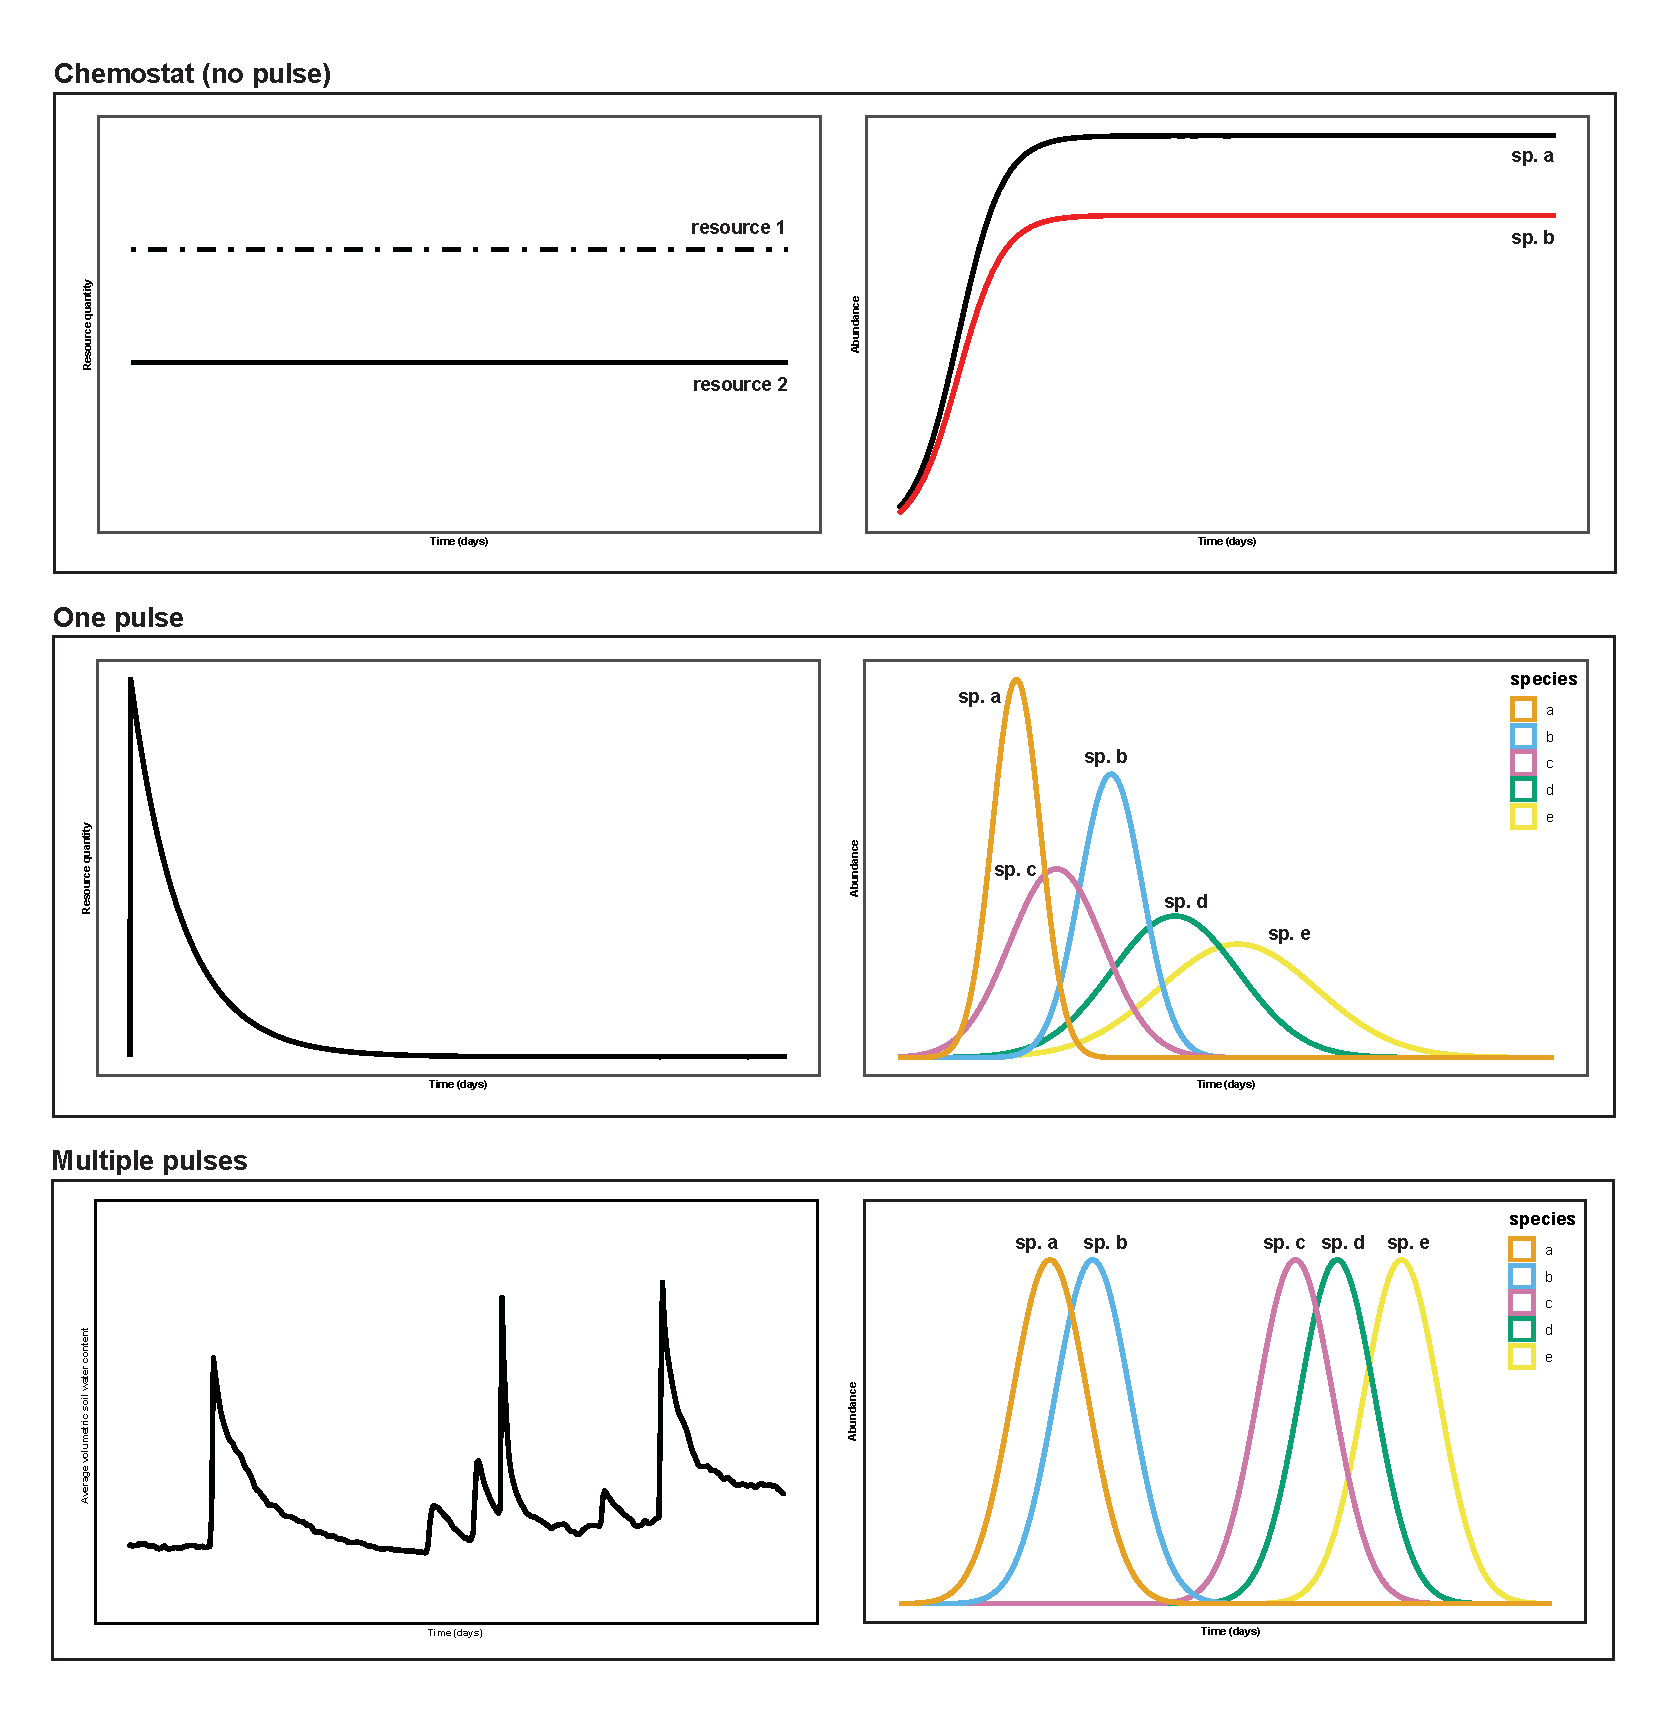
\includegraphics[width=0.8\textwidth]{..//figures/JN_conceptfigs/sixpanel_concept.png}
\caption{Theory suggests resource levels may determine temporal niche space. In a system where resources are constant (top left,, chemostat; species can only coexist if they are each equally good competitors for different resources) species would be expected to show little temporal fluctuations and there would be no real temporal niches. Many models of coexistence today, however, assume a resource pulse that decays (middle, left; e.g., water with evaporative loss, such as in snowpack systems) over time: this resource then sets the temporal window of each season and species compete within it. Most real systems however are more complicated (bottom left, taken from Jornada LTER site 302 showing soil moisture at 10 cm depth over the year) ....} 
% Evaporating single pulse resource: species may invade only at certain levels of resource (includes snowpack/soil nutrients etc.)
%  Multiple pulses: Some species may persist through whole season or use first or second pulse only
 \label{fig:resource}
\end{figure}



\end{document}
